
%(BEGIN_QUESTION)
% Copyright 2006, Tony R. Kuphaldt, released under the Creative Commons Attribution License (v 1.0)
% This means you may do almost anything with this work of mine, so long as you give me proper credit

How could the following pneumatic controller mechanism be altered to make the ``bias'' term adjustable? 

$$\includegraphics[width=15.5cm]{i01480x01.eps}$$

\underbar{file i01480}
%(END_QUESTION)





%(BEGIN_ANSWER)

$$\includegraphics[width=15.5cm]{i01480x02.eps}$$

%(END_ANSWER)





%(BEGIN_NOTES)

Bias is provided by the spring pulling down on the lever.  To make it adjustable, the spring tension may be connected to a screw that can be moved.  You should remind your students that the bias term is {\it added} to the proportional term of the controller, and as such must be a force added to (or subtracted from) forces in the force-balance system.

%INDEX% Control, proportional: pneumatic controller bias adjustment

%(END_NOTES)


